\section{Exact loop blocks and learned costs through thirteen loops}
\label{sec:blocks13}
The next extension changes the calculation around the learned choice. When the active propagators and numerators divide the loop momenta into independent blocks, we reduce each distinct block once and keep the product of its master expansions in factored form. Shared external momenta do not prevent this separation. An active numerator that joins two loop sets prevents their separate reduction. Appendix~\ref{app:blocks13} derives the factorization and gives exact tadpole, one-mass vacuum, and massless two-point formulas used before native Kira. These routes use mathematical identities and make no learned choice.

The remaining blocks use the same 44 structural inputs and ten seed actions as the shared model. We fit eleven new candidates on all 111 available historical training requests, with 76 separate validation requests. They comprise six forests, two regularized linear regressions, and three neural networks. The forests follow the random-forest and extremely randomized-tree methods~\cite{Breiman2001Forest,Geurts2006ExtraTrees}. Each forest averages its tree predictions. The cost labels sum the native attempts and their recovery cost, since a checked stored basis permits a single production reduction. An unsuccessful full action receives a penalty. The first selection retains the preceding network with two 48-component hidden layers. After adding the two exact convolution formulas, we compare the fitted candidates again on the historical validation requests that still need native Kira, and retune the fixed control on the same requests. This final selection precedes the corrected reserved test. The notes give the candidate settings and selection rules.

A stored basis contains integral indices, and Kira recomputes coefficients at the current parameters. During development, combining several alternative preferred master lists allowed different seed actions to return different bases. Their coefficients could not be compared entry by entry. We therefore reduce all stored preferred indices at separate development parameters and retain one checked master set per structure. A production result must use this set; otherwise the application retries with less restrictive seeds. Unknown structures require master discovery and a second exact calculation. These preparation costs remain outside the supplied-cache timing and are recorded separately in the notes.

The first reserved grid contains 79 coupled-family requests and 52 independent-block requests through thirteen loops. It records every failure and native input limit. After the basis correction, we use new parameter profiles for the coupled and product tests. Each product uses one- or two-loop blocks; a total of thirteen loops therefore tests the exact composition and its local learned decisions. It does not test a general irreducible thirteen-loop matrix. Further sets check the derived one-mass vacuum and massless two-point formulas with scalar targets and one quadratic numerator. The notes give the initial grid and all outcomes, while Table~\ref{tab:blocks13} gives the corrected application's paired results.

All three corrected methods share the block construction, exact formulas, checked basis, and recovery limits. The native method uses native seed bounds. The fixed method uses the preselected common action. The learned method predicts an action from the block structure. Each timing starts a fresh process and includes prediction, native equation generation, reduction, recovery, output, and exact comparison with an independent reference. Three repetitions rotate method order. Reference preparation is separate. A time ratio uses only requests for which both methods complete all three exact checks; incomplete requests remain in the coverage counts. Analytic-only requests contribute no evidence for ML.

The final validation comparison contains 58 requests that need native Kira and 18 requests handled by the exact formulas. It selects a 48-tree extremely randomized forest with maximum depth 10, with decision margin 0.0. The model weights and decision rule remain fixed throughout the corrected reserved tests.

The corrected grid contains 92 requests. The learned route completes all three exact checks on 91 of them, with 0 first-run completions that lack matching reference coefficients. Across all methods, the experiment records 892 timed attempts and 38012 coefficient comparisons.

\begin{table}[!htbp]\centering\small
\caption{Corrected application: paired time ratios on completed requests. The numerator is the learned application time; the controls share all exact changes. Times are sums of request medians in seconds. Each row has its own matched set. Analytic rows execute the same formula code and contain no ML inference. These are measurements of this study.}
\label{tab:blocks13}
\begin{tabularx}{\linewidth}{@{}Yrrrr@{}}\toprule
Comparison & Requests & Control & Learned & Ratio\\\midrule
Coupled families / native & 18 & 27.400 & 22.715 & 0.829\\
Coupled families / fixed & 18 & 22.471 & 22.715 & 1.011\\
Independent blocks / native & 52 & 187.116 & 189.802 & 1.014\\
Independent blocks / fixed & 52 & 191.693 & 189.802 & 0.990\\
Vacuum formula / native & 11 & 12.441 & 11.300 & 0.908\\
Vacuum formula / fixed & 11 & 11.735 & 11.300 & 0.963\\
Massless formula / native & 10 & 10.895 & 10.796 & 0.991\\
Massless formula / fixed & 10 & 10.866 & 10.796 & 0.994\\
\bottomrule\end{tabularx}\end{table}
\begin{figure}[!htbp]\centering
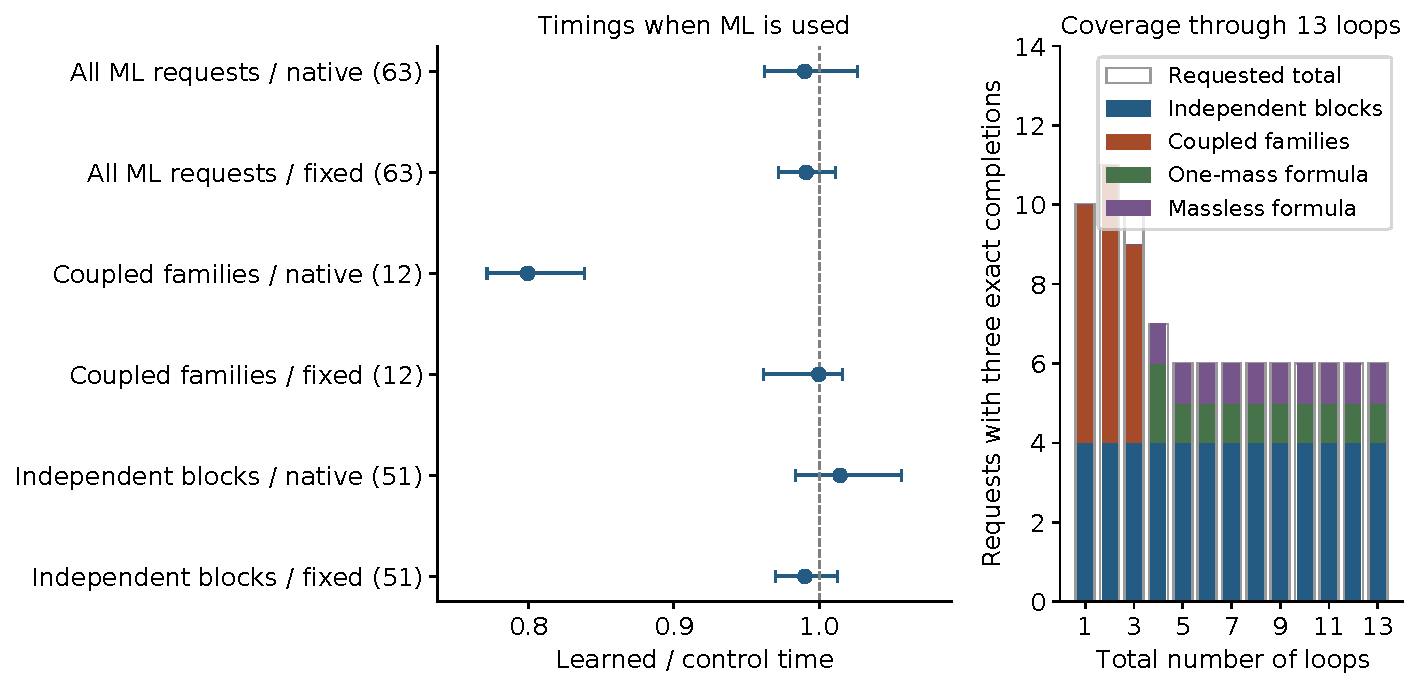
\includegraphics[width=\linewidth]{paper_figures/factorized_results.pdf}
\caption{Left: only requests that invoke ML are included, and the controls share all exact changes. The comparisons with fixed choices include equal time within repetition variation. Intervals describe the three repetitions. Counts in parentheses identify matched requests. Right: completion depends on the integral structure. High-loop products contain small independent blocks, while each analytic formula applies to its specified denominator structure. The bar outline gives the requested total. These sets do not establish general coupled high-loop coverage.}
\label{fig:blocks13}\end{figure}

On requests that actually invoke ML, the time ratio is 0.990, with repetition interval $[0.963,1.026]$, on 63 matched requests. Against the fixed action on its matched ML requests, the time ratio is 0.991, with repetition interval $[0.972,1.011]$, on 63 matched requests. The comparison with native choices does not resolve a saving beyond repetition variation. The comparison with fixed choices does not resolve a saving beyond repetition variation. These controls isolate the learned seed decision after the exact changes.

The learned method records 45 unsuccessful native attempts among 288 native calls in the timed tests. A completed request includes its failed attempts and recovery in the measured cost. Unverified learned attempts consume 101.255 seconds in addition to the paired completed-request totals. Their outcomes remain in the coverage counts.

Across all timed attempts, the learned application uses 811.364 seconds, native choices use 790.074 seconds, and the fixed choice uses 818.950 seconds. This total includes the unfinished request and all repetitions. The learned application therefore does not reduce total time against native choices on this bounded workload.

In the 63 matched ML requests against the fixed control, the model changes the first native action in 34 requests. The remaining requests retain the fixed action and still pay the prediction cost.

Compared with the initial block application on the matched fresh coupled set, the time ratio is 1.046, with repetition interval $[0.989,1.085]$, on 16 matched requests. On the separate one-mass vacuum targets with a completed initial block reduction, the time ratio is 0.187, with repetition interval $[0.168,0.214]$, on 4 matched requests. For the corresponding massless numerator comparison, the time ratio is 0.781, with repetition interval $[0.724,0.891]$, on 1 matched requests. These changes include exact formulas and revised basis handling, so they do not measure ML alone.

The separate gamma-formula checks cover 14 vacuum requests through thirteen loops and 50 target coefficients. Native Kira confirms 5 of the attempted low-loop requests, with 14 coefficient comparisons; 0 attempted native references do not complete. Higher-loop agreement between the finite-product and gamma expressions checks the derivation and implementation, without establishing a native high-loop timing gain.
\FloatBarrier

The massless numerator checks add 12 requests and 60 gamma comparisons through thirteen loops. Native Kira verifies 3 low-loop requests and 15 coefficients; 0 native references do not complete. These formulas precede ML and provide no evidence for a learned gain.
